\chapter{Streams}

\begin{summary}
De Stream API van Java biedt een elegante manier om collections te manipuleren. De belangrijkste interface uit de API is Stream$<$T$>$. Als Java ontwikkelaar gebruik je voornamelijk deze interface die alle implementatie-details verbergt. Bij het ontwerpen van de Stream API is, naast het aanbieden van een elegante en eenvoudige API, ook veel aandacht besteed aan performantie. 
\end{summary}

\section{External en internal iterators}

Veronderstel dat we een verzameling met Movie-objecten hebben: \textit{movies}. We willen nu graag weten hoeveel actiefilms er in onze verzameling zitten.

Hier is de code om dit te berekenen.

\begin{lstlisting}
int count = 0;
for (Movie movie: movies) {
    if (movie.getGenre() == Genre.ACTION) {
        count++;
    }
}
\end{lstlisting}

Bovenstaand voorbeeld bevat veel boilerplate code en daarnaast hebben we ook een external iterator. 

Een stream maakt het mogelijk om op een functionele manier complexe bewerkingen uit te voeren op een verzameling.
We kunnen bovenstaande code schrijven met behulp van een stream. Onze external iterator verdwijnt en we krijgen een internal iterator in de plaats.

\begin{lstlisting}
int count = movies.stream().filter(m -> m.getGenre() == Genre.ACTION).count();
\end{lstlisting}

Een stream bestaat uit 3 delen: een (data) bron, intermediate operations (tussentijdse bewerkingen) en een terminal operation (eindbewerking). In ons voorbeeld is de verzameling movies de bron, vervolgens hebben we een intermediate operation \textit{filter} en tenslotte een terminal operation \textit{count}.

\begin{figure}[H]
  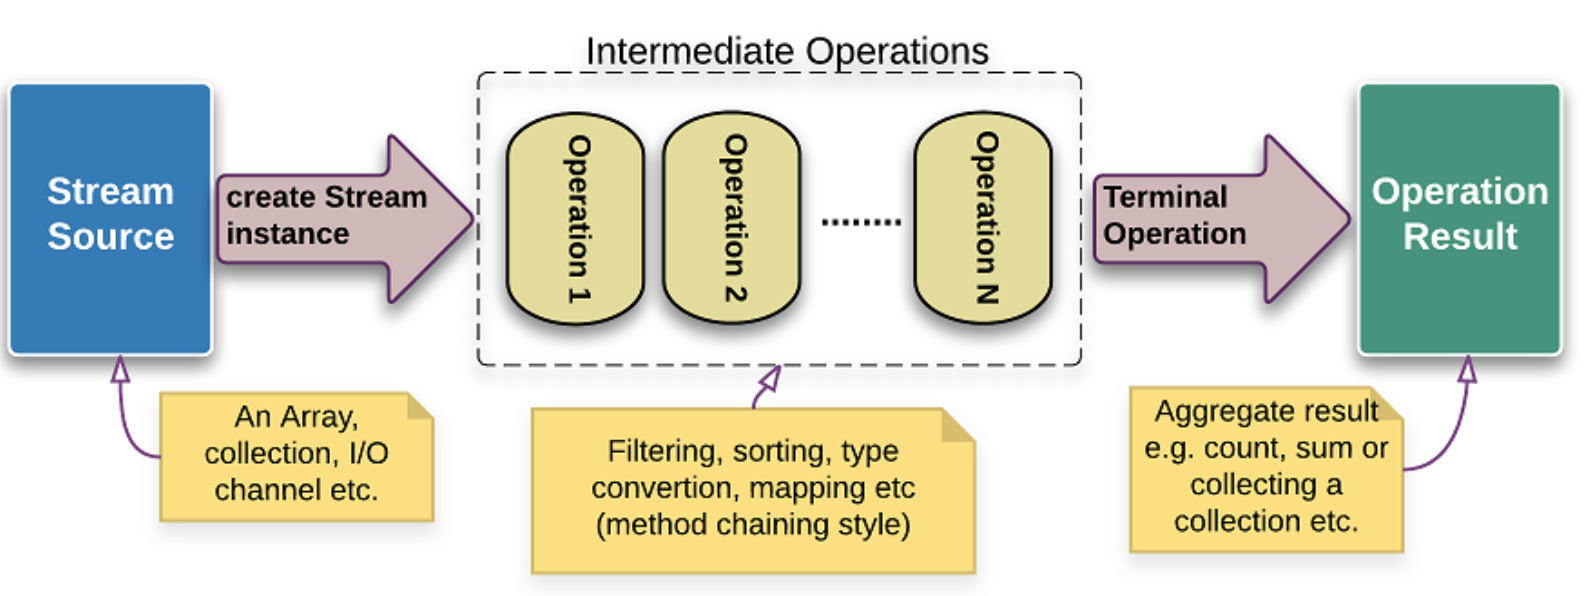
\includegraphics[width=\linewidth]{images/chapter_streams/stream_pipeline.png}
  \caption{Stream pipeline (logicbig.com)}
  \label{fig:stream_of}
\end{figure}


De intermediate operators verwerken de elementen van de stream \'e\'en voor \'e\'en. Alle intermediate operations zijn lui (lazy), ze worden enkel uitgevoerd als de stream wordt afgesloten door een terminal operation.

De internal iterator geniet meestal de voorkeur. Internal iterations kunnen korter geschreven worden en zijn daardoor ook makkelijker lees- en onderhoudbaar. Toch zijn er situaties, zoals wanneer je 2 verzamelingen gelijktijdig manipuleert, dat je kiest voor een external iterator.

\begin{figure}[H]
  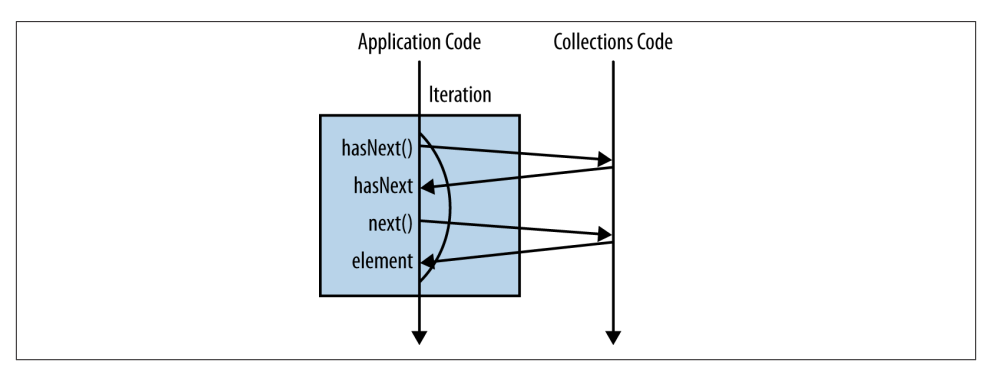
\includegraphics[width=\linewidth]{images/chapter_streams/external_iteration.png}
  \caption{External iteration}
  \label{fig:external_iteration}
\end{figure}

\begin{figure}[H]
  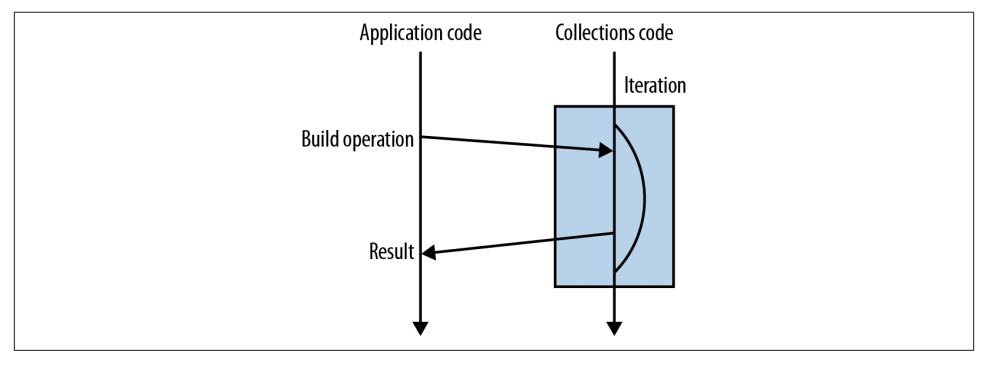
\includegraphics[width=\linewidth]{images/chapter_streams/internal_iteration.png}
  \caption{Internal iteration}
  \label{fig:internal_iteration}
\end{figure}

\section{Intermediate en terminal operations}

\subsection{Terminal operation .collect()}

\begin{lstlisting}
import java.util.List;
import java.util.stream.Collectors;
import java.util.stream.Stream;

public class DemoCollect {

	public static void main(String[] args) {

		List<String> theBeatles = 
				Stream.of("John Lennon", "Paul McCartney", "George Harrison", "Ringo Starr")
				.collect(Collectors.toList());
		System.out.println(theBeatles);
	}

}
\end{lstlisting}

Een stream is geen datastructuur of verzameling. Je moet een stream zien als een reeks objecten. E\'en van de manieren om zo'n reeks of stream te bouwen is met de static methode \textit{of} van de interface Stream.

\begin{figure}[H]
  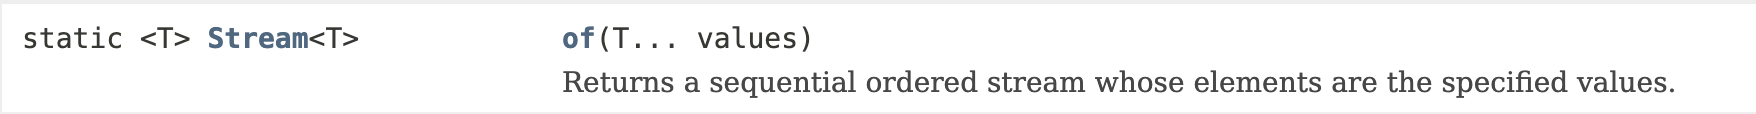
\includegraphics[width=\linewidth]{images/chapter_streams/stream_of.png}
  \caption{Static methode of() in de interface Stream}
  \label{fig:stream_of}
\end{figure}

Door gebruik te maken van de operation \textit{collect(Collectors.toList())} kunnen we de objecten uit de stream verzamelen in een List.

\subsection{Intermediate operation .filter()}

Wanneer je bepaalde elementen uit een stream wil selecteren, gebruik je een filter. 

\begin{figure}[H]
  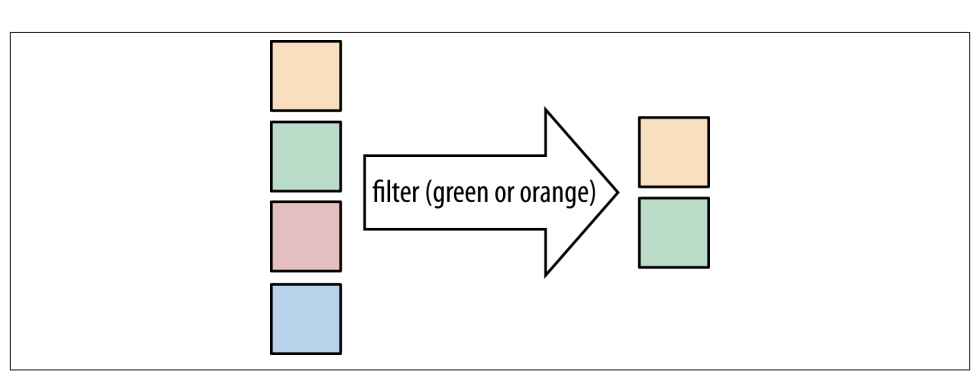
\includegraphics[width=\linewidth]{images/chapter_streams/illustration_filter.png}
  \caption{Filter operation}
  \label{fig:filter_operation}
\end{figure}

\begin{figure}[H]
  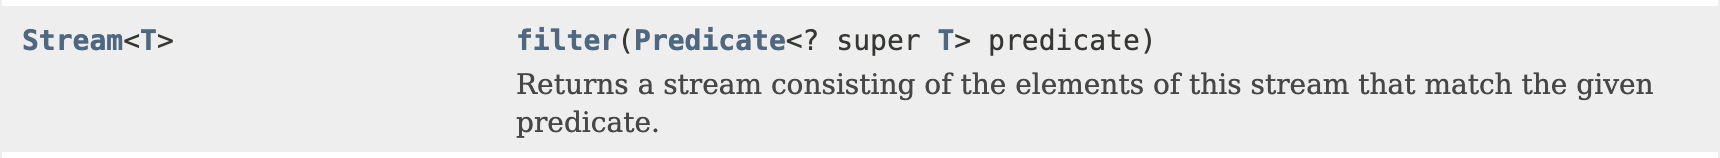
\includegraphics[width=\linewidth]{images/chapter_streams/stream_filter.png}
  \caption{Methode filter() in de interface Stream}
  \label{fig:stream_filters}
\end{figure}

Aan de hand van een Predicate wordt beslist welke elementen geselecteerd worden. 

In het onderstaande voorbeeld selecteren we de even getallen uit de verzameling numbers.

\begin{lstlisting}
List<Integer> numbers = Arrays.asList(1,2,3,4,5);

List<Integer> evenNumbers = numbers.stream()
				.filter(n -> n%2  == 0)
				.collect(Collectors.toList());
				
assertEquals(Arrays.asList(2,4), evenNumbers);
\end{lstlisting}

Nog een voorbeeld.

\begin{lstlisting}
List<String> animals = Stream.of("zebra", "dog", "dolphine")
				.filter(a -> a.contains("o"))
				.collect(Collectors.toList());

assertEquals(Arrays.asList("dog", "dolphine"), animals);
\end{lstlisting}

Alle String-objecten die een ``o'' bevatten mogen in de stream aanwezig blijven.

Merk op dat de functie filter() een intermediate operation is. De bewerking heeft als return-type Stream. We bouwen als het ware een pipeline. De filter()-operation is ook lazy en zal pas effectief uitgevoerd worden als er een terminal-operation aanwezig is.

Hier volgt nog een voorbeeld met een verzameling met objecten van een zelfgeschreven klasse Participant.

\begin{lstlisting}
public class Participant {
	private String name;
	private int points;

	public Participant(String name, int points) {
		this.name = name;
		this.points = points;
	}

	public int getPoints() {
		return points;
	}

	public String getName() {
		return name;
	}
}
\end{lstlisting}

\begin{lstlisting}
Participant john = new Participant("John P.", 15);
Participant sarah = new Participant("Sarah M.", 200);
Participant charles = new Participant("Charles B.", 150);
Participant mary = new Participant("Mary T.", 1);

List<Participant> participants = Arrays.asList(john, sarah, charles, mary);

List<Participant> over100Points = participants.stream()
     .filter(p -> p.getPoints() > 100)
     .collect(Collectors.toList());

assertEquals(Arrays.asList(sarah, charles), over100Points);
\end{lstlisting}

Je kan ook meerdere criteria gebruiken in een filter. Je kan in het Predicate de verschillende criteria samenvoegen via boolean operatoren.

\begin{lstlisting}
List<Participant> selection = participants.stream()
    .filter(p -> p.getPoints() > 100 && p.getName().startsWith("S"))
    .collect(Collectors.toList());
    
assertEquals(Collections.singletonList(sarah), selection);
\end{lstlisting}

Daarnaast kan je ook gebruikmaken van methodes als ``or'',  ``and'' en ``negate'' uit de interface Predicate.
		
\begin{lstlisting}
Predicate<Participant> over100Points = p -> p.getPoints() > 100;
Predicate<Participant> startingWithS = p -> p.getName().startsWith("S");

List<Participant> selection = participants.stream()
    .filter(over100Points.and(startingWithS))
    .collect(Collectors.toList());

assertEquals(Collections.singletonList(sarah), selection);
\end{lstlisting}

\subsection{Terminal operation .forEach()}

De methode .forEach() is een terminal operation en aanvaardt een implementatie van de functionele interface Consumer als parameter. Deze Consumer beschrijft een actie die met ieder element van de verzameling uitgevoerd zal worden.

\begin{figure}[H]
  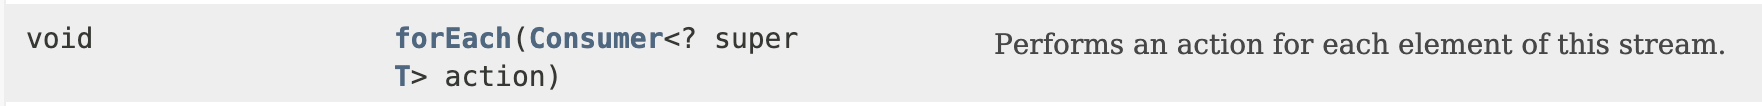
\includegraphics[width=\linewidth]{images/chapter_streams/stream_forEach.png}
  \caption{Methode forEach() in de interface Stream}
  \label{fig:stream_foreach}
\end{figure}

\begin{lstlisting}
public class DemoForEach {

	public static void main(String[] args) {
		Participant john = new Participant("John P.", 15);
		Participant sarah = new Participant("Sarah M.", 200);
		Participant charles = new Participant("Charles B.", 150);
		Participant mary = new Participant("Mary T.", 1);

		List<Participant> participants = Arrays.asList(john, sarah, charles, mary);

		participants.stream()
		    .filter(p -> p.getPoints() >= 200)
		    .forEach(System.out::println);

		System.out.println("* All participants *");

		participants.forEach(System.out::println);
	}
}
\end{lstlisting}

Iedere Collection biedt via de interface Iterable ook een forEach methode aan. Met beide forEach functies kan je hetzelfde resultaat bereiken.

\begin{lstlisting}
participants.forEach(System.out::println);
participants.stream().forEach(System.out::println);
\end{lstlisting}

Toch gaat in dit geval onze voorkeur uit naar de eerste optie. Omdat we hier itereren over alle elementen is de stream overbodig.


\subsection{Intermediate operation .map()}

Als je een functie hebt om objecten van \'e\'en datatype te transformeren naar een ander datatype, dan kan je met de bewerking .map(), deze functie loslaten op alle objecten van een stream. 

\begin{figure}[H]
  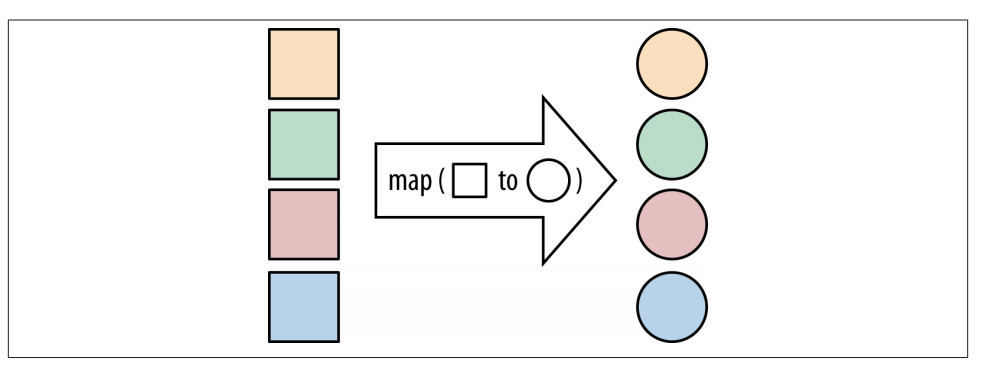
\includegraphics[width=\linewidth]{images/chapter_streams/illustration_map.png}
  \caption{Map operation}
  \label{fig:stream_foreach}
\end{figure}

\begin{figure}[H]
  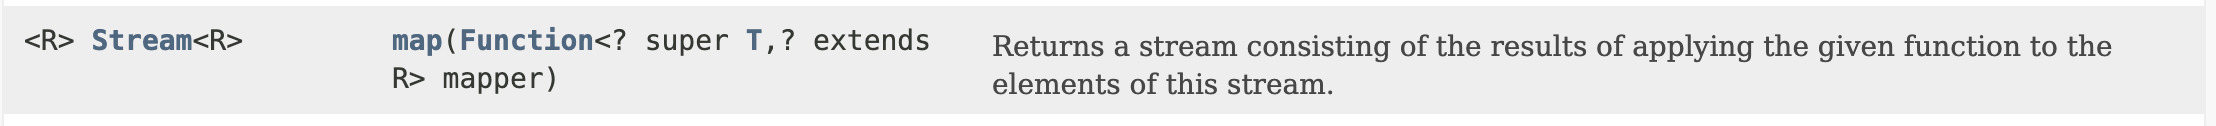
\includegraphics[width=\linewidth]{images/chapter_streams/stream_map.png}
  \caption{Methode map() in de interface Stream}
  \label{fig:stream_foreach}
\end{figure}

Map is een lazy operator. Zonder terminal operator zal de meegegeven functie niet uitgevoerd worden, en zal je dus ook geen resultaat krijgen. De functie die je meegeeft aan map is een implementatie van de generieke functionele interface Function$<$T,R$>$.

Hier volgen een twee voorbeelden. In het eerste voorbeeld wijzigt het datatype van de elementen van de stream niet. In het tweede voorbeeld wordt ieder String-object in de stream vervangen door een Integer-waarde.

\begin{lstlisting}
List<String> animals = Stream.of("zebra", "dog", "dolphine")
				.map(String::toUpperCase)
				.collect(Collectors.toList());

assertEquals(Arrays.asList("ZEBRA", "DOG", "DOLPHINE"), animals);
\end{lstlisting}

\begin{lstlisting}
List<Integer> lengths = Stream.of("zebra", "dog", "dolphine")
				.map(String::length)
				.collect(Collectors.toList());

assertEquals(Arrays.asList(5, 3, 8), lengths);
\end{lstlisting}

\subsection{Intermediate operation .sorted()}

Wanneer je de intermediate operation sorted() toevoegt aan een stream, worden de elementen in de stream gesorteerd. Zonder parameter zal sorted() de natuurlijke sortering gebruiken. Voor objecten van een zelfgeschreven klasse zorg je er dus voor dat de interface Comparable ge\"implementeerd wordt.

Het is ook mogelijk dat je aan de functie sorted() een parameter meegeeft waarmee je een andere volgorde kan afdwingen. In het tweede voorbeeld gebruiken we niet de natuurlijke (alfabetische) volgorde, maar worden de woorden van lang naar kort gesorteerd.


\begin{lstlisting}
List<String> sortedList = Stream.of("zebra", "dog", "dolphine")
				.sorted()
				.collect(Collectors.toList());

assertEquals(Arrays.asList("dog", "dolphine", "zebra"), sortedList);
\end{lstlisting}

\begin{lstlisting}
List<String> sortedList = Stream.of("zebra", "dog", "dolphine")
				.sorted((x, y) -> y.length() - x.length())
				.collect(Collectors.toList());
		
assertEquals(Arrays.asList("dolphine", "zebra", "dog"), sortedList);
\end{lstlisting}

\subsection{Intermediate operation .distinct()}

De operation .distinct() zorgt ervoor dat de elementen in de stream uniek zijn. Elementen die meermaals voorkomen worden verwijderd. Het is de implementatie van de equals() methode (en dus ook hashCode()) van een klasse die beslist of de elementen uniek zijn of niet.

\begin{lstlisting}
List<String> withoutDoubles = Stream.of("zebra", "dog", "zebra", "dolphine")
    .distinct()
    .collect(Collectors.toList());
    
assertEquals(3, withoutDoubles.size());
\end{lstlisting}

\subsection{Intermediate operation .limit()}

De operation .limit() heeft 1 parameter die het maximaal toegelaten elementen in de stream geeft.
De stream wordt dus als het ware afgekapt.

\begin{lstlisting}
List<String> animals = Stream.of("zebra", "dog", "elephant", "camel", "cat", "fish","dolphine")
    .limit(4)
    .collect(Collectors.toList());
assertEquals(4, animals.size());
\end{lstlisting}

Met de methode iterate kunnen we een oneindige stream maken. Dankzij de limit(5) worden slechts de eerste 5 nummers gegenereerd.

\begin{lstlisting}
List<Integer> numbers = Stream.iterate(1, n -> n + n)
    .limit(5)
    .collect(Collectors.toList());

assertEquals(Arrays.asList(1,2,4,8,16), numbers);
\end{lstlisting}


\subsection{Intermediate operation peek()}

De intermediate operation peek kan gebruikt worden om je pipeline te debuggen. Als je wilt controleren welke elementen er op een gegeven moment in de pipeline zitten, dan voeg je peek toe. Zolang je geen terminal operation hebt toegevoegd zal ook peek geen resultaat laten zien.

\begin{lstlisting}
Stream.of("one", "two", "three", "four")
  .filter(e -> e.length() > 3)
  .peek(e -> System.out.println("Filtered value: " + e))
  .map(String::toUpperCase)
  .peek(e -> System.out.println("Mapped value: " + e))
  .collect(Collectors.toList());
\end{lstlisting}

Je kan de operation peek() verder ook handig gebruiken om de elementen van je stream aan te passen.

\begin{lstlisting}
Stream<User> userStream = Stream.of(new User("Alice"), new User("Bob"), new User("Chuck"));
userStream.peek(u -> u.setName(u.getName().toLowerCase()))
  .forEach(System.out::println);
  \end{lstlisting}


\subsection{Terminal operation .count()}

\begin{lstlisting}
long over100Points = participants.stream().filter(p -> p.getPoints() > 100).count();

assertEquals(2, over100Points);
\end{lstlisting}
		
De terminal operation count gebruik je om het aantal elementen in de stream te tellen.
Indien je geen gebruik maakt van intermediate operations gebruik je de methode size() van je collection om het aantal elementen te achterhalen.

\begin{lstlisting}
System.out.println("Number of participants: " + participants.size());
\end{lstlisting}
		
\section{Intstream, LongStream en DoubleStream}
	
Er zijn ook een aantal afgeleide interfaces van de interface Stream. Deze bieden extra functionaliteit aan. Zo hebben we bijvoorbeeld de interface IntStream, die speciaal ontworpen is voor streams met gehele getallen. Deze stream bevat elementen met datatype \textit{int}. Naast IntStream hebben we ook de interfaces DoubleStream en LongStream. Al deze interfaces bevatten de methoden sum(), min(), max() en average(). 

\subsection{sum()}

Met de operation sum kan je eenvoudig de som berekenen van alle elementen in je stream.

\begin{lstlisting}
long totalPoints = participants.stream().mapToInt(Participant::getPoints).sum();

assertEquals(366, totalPoints);
\end{lstlisting}
		

\subsection{range() en rangeClosed()}
		
De static methoden range() en rangeClosed() zijn beschikbaar in de interfaces java.util.stream.IntStream en java.util.stream.LongStream. Je kan ze gebruiken om een stream te cre\"eren met gehele getallen vanaf een init\"ele waarde tot een stop waarde.
\begin{figure}[H]
  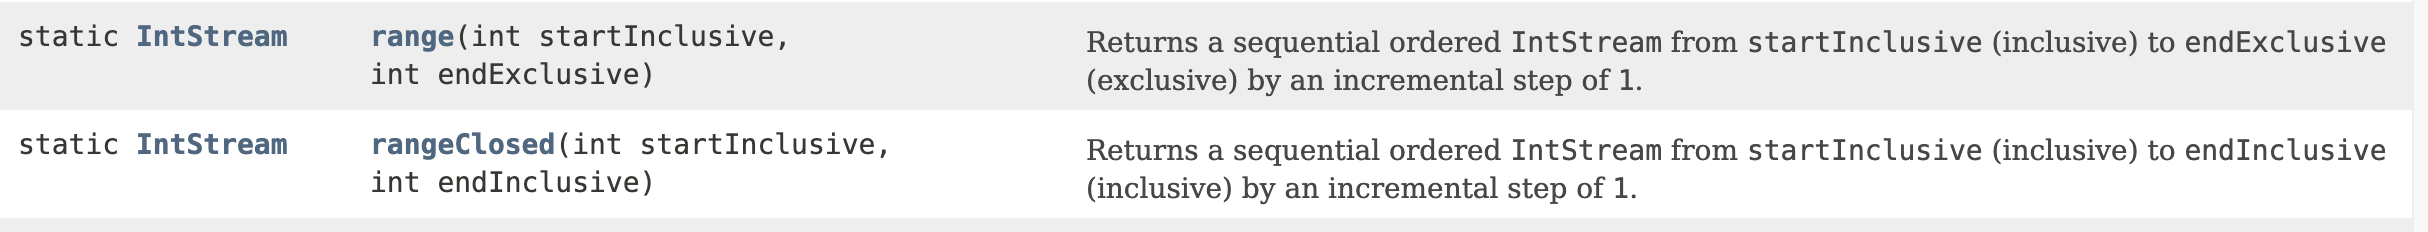
\includegraphics[width=\linewidth]{images/chapter_streams/intstream_range.png}
  \caption{Aanmaken van IntStream met range() of rangeClosed()}
  \label{fig:stream_foreach}
\end{figure}

\begin{lstlisting}
long count = IntStream.rangeClosed(10, 20).count();

assertEquals(11, count);
\end{lstlisting}

\subsection{min(), max() en average()}

\begin{figure}[H]
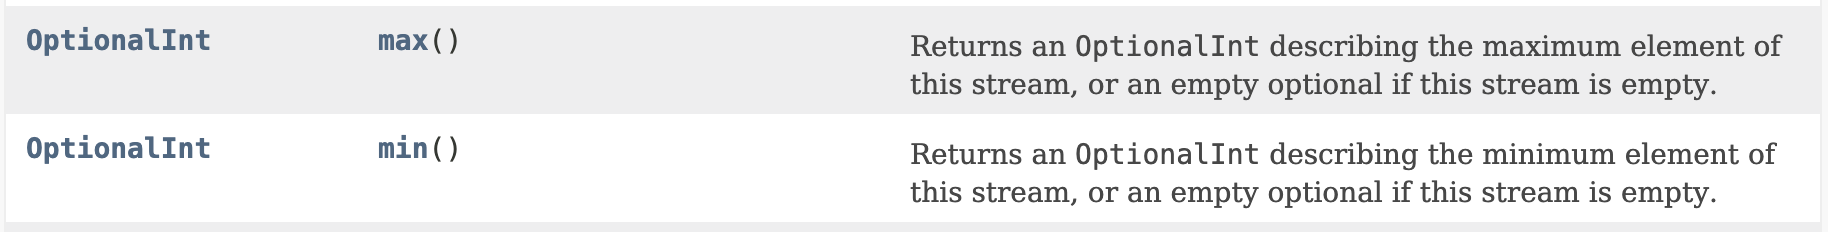
\includegraphics[width=\linewidth]{images/chapter_streams/intstream_max_min.png}
\caption{min() en max() uit de interface IntStream}
\label{fig:instream_min_max}
\end{figure}

\begin{figure}[H]
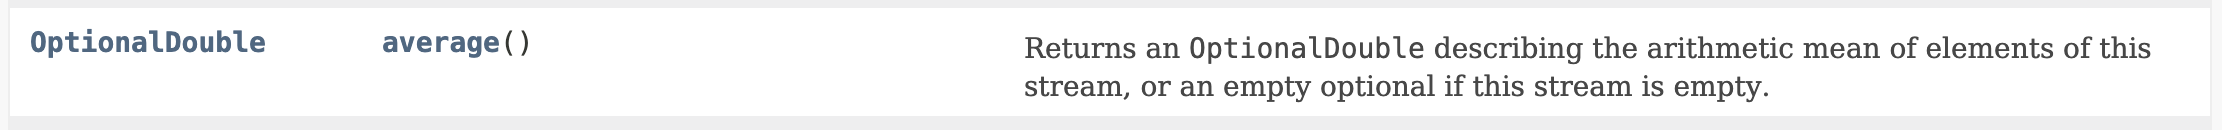
\includegraphics[width=\linewidth]{images/chapter_streams/intstream_average.png}
\caption{average() uit de interface IntStream}
\label{fig:instream_average}
\end{figure}

Merk op dat de methoden max() en min() een object van de klasse OptionalInt als return-type hebben. De methode average() heeft OptionalDouble als return-type. 

\begin{oefening}
Zoek de klasse OptionalInt en OptionalDouble op in de Java documentatie.
\end{oefening}

In de documentatie vind je terug dat dit een container-object is dat een int- of double-waarde kan bevatten. Indien we namelijk een lege stream hebben, dan bestaat er immers geen minimum, maximum of gemiddelde. In plaats van bijvoorbeeld een exception op te gooien wanneer we max() oproepen voor een lege IntStream, is er gekozen om steeds een OptionalInt als resultaat te geven. Bij een lege IntStream bevat het OptionalIInt-object geen waarde en \textit{isPresent()} geeft false als resultaat. Indien er wel een maximum berekend kan worden geeft \textit{isPresent()} true. De berekende waarde kan je bekomen via de methode \textit{getAsInt()}.

\begin{lstlisting}
Random random = new Random();
List<Integer> randomNumbers = random.ints(15, 0, 100).boxed().collect(Collectors.toList());
int max = randomNumbers.stream().mapToInt(x -> x).max().getAsInt();
int min = randomNumbers.stream().mapToInt(x -> x).min().getAsInt();
double average = randomNumbers.stream().mapToInt(x -> x).average().getAsDouble();
assertTrue(min <= average);
assertTrue(max >= average);

IntSummaryStatistics intSummaryStatistics = random.ints(15, 0, 100).summaryStatistics();
assertTrue(intSummaryStatistics.getMax() >= intSummaryStatistics.getMin());
\end{lstlisting}


\begin{oefening}
Wil je eens aan de slag met de klasse Optional, dan kan je de volgende oefening maken op CodinGame:\\
\url{https://www.codingame.com/playgrounds/20782/java-guild-meeting-52018/optionals---practice}.
\end{oefening}